\documentclass{article}

\usepackage{tikz}
\usetikzlibrary{automata,arrows,calc,positioning}
\usetikzlibrary{shapes,shapes.geometric}
\tikzset{state/.style={
        draw,
        circle,
        minimum size=1.25cm,
    }
}

\usepackage[margin=1in]{geometry}

\begin{document}

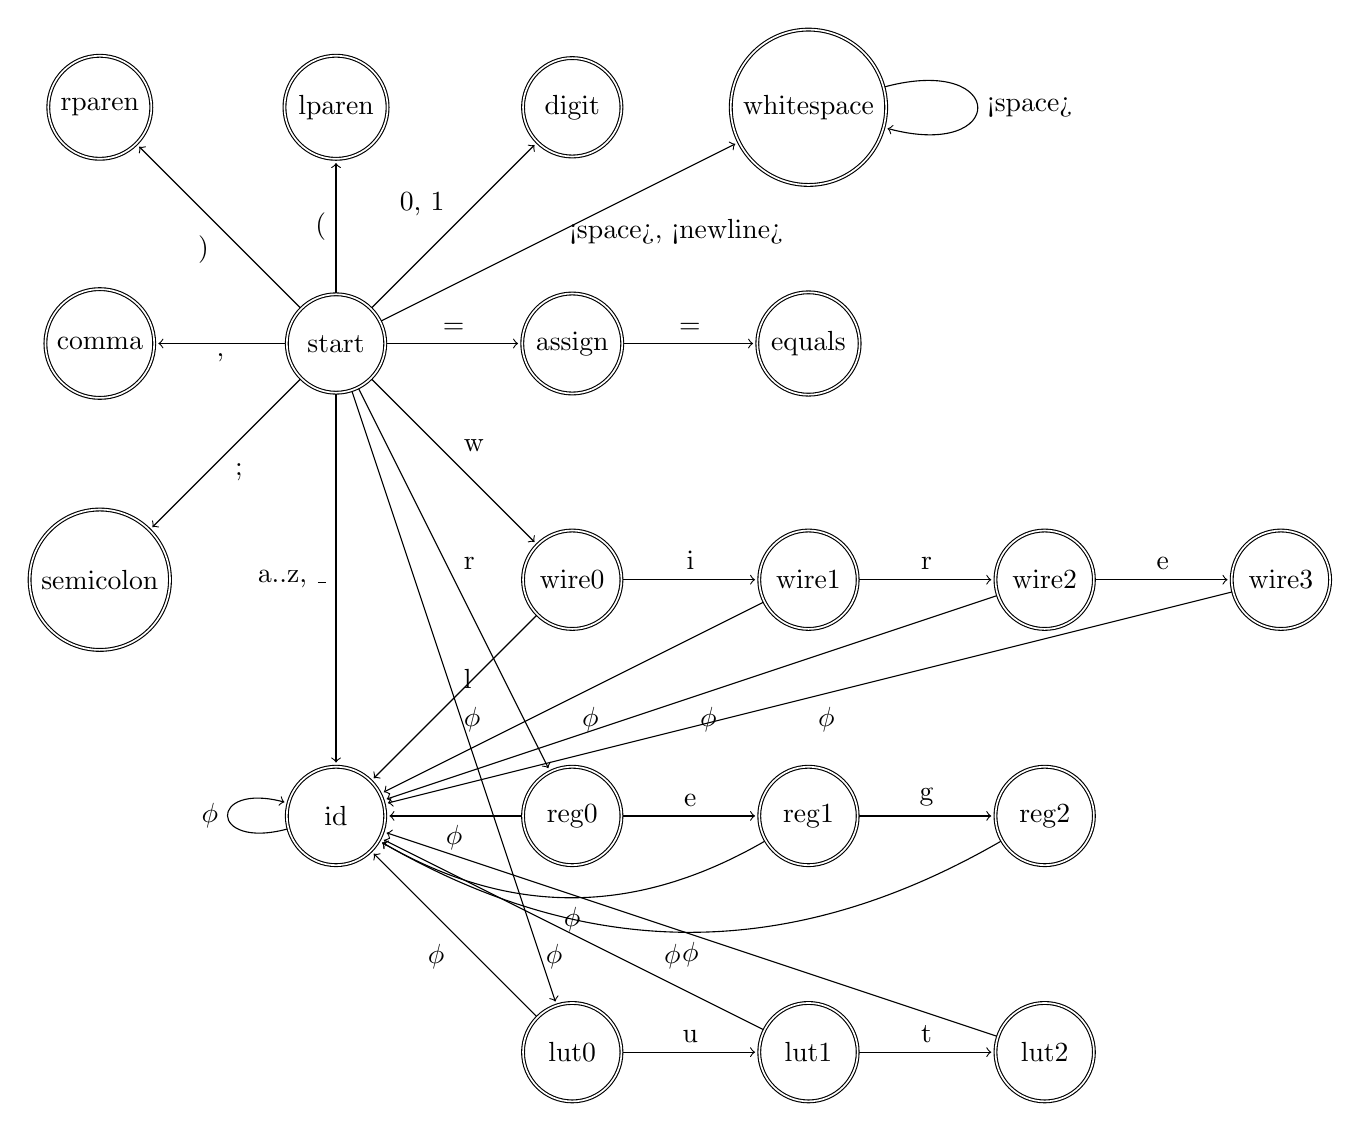
\begin{tikzpicture}[shorten >=1pt,node distance=3cm,on grid,auto]
  \node[state, accepting] (start)   {start};
  \node[state, accepting] (lparen) [above=of start] {lparen};
  \node[state, accepting] (rparen) [left=of lparen] {rparen};
  \node[state, accepting] (assign) [right=of start] {assign};
  \node[state, accepting] (equals) [right=of assign] {equals};
  \node[state, accepting] (digit) [right=of lparen] {digit};
  \node[state, accepting] (whitespace) [right=of digit] {whitespace};
  \node[state, accepting] (comma) [below=of rparen] {comma};
  \node[state, accepting] (semicolon) [below=of comma] {semicolon};
  \node[state, accepting] (wire0) [below=of assign] {wire0};
  \node[state, accepting] (wire1) [right=of wire0] {wire1};
  \node[state, accepting] (wire2) [right=of wire1] {wire2};
  \node[state, accepting] (wire3) [right=of wire2] {wire3};
  \node[state, accepting] (reg0) [below=of wire0] {reg0};
  \node[state, accepting] (reg1) [right=of reg0] {reg1};
  \node[state, accepting] (reg2) [right=of reg1] {reg2};
  \node[state, accepting] (lut0) [below=of reg0] {lut0};
  \node[state, accepting] (lut1) [right=of lut0] {lut1};
  \node[state, accepting] (lut2) [right=of lut1] {lut2};
  \node[state, accepting] (id) [left=of reg0] {id};
  \path[->]
  (start)
  edge node {0, 1} (digit)
  edge node {=} (assign)
  edge node {(} (lparen)
  edge node {)} (rparen)
  edge node {,} (comma)
  edge node {;} (semicolon)
  edge [left] node {a..z, \_} (id)
  edge node {w} (wire0)
  edge node {r} (reg0)
  edge node {l} (lut0)
  edge [right] node {<space>, <newline>} (whitespace)
  (assign)
  edge node {=} (equals)
  (wire0)
  edge node {i} (wire1)
  edge node {$\phi$} (id)
  (wire1)
  edge node {r} (wire2)
  edge node {$\phi$} (id)
  (wire2)
  edge node {e} (wire3)
  edge node {$\phi$} (id)
  (wire3)
  edge node {$\phi$} (id)
  (reg0)
  edge node {e} (reg1)
  edge node {$\phi$} (id)
  (reg1)
  edge node {g} (reg2)
  edge [bend left] node {$\phi$} (id)
  (reg2)
  edge [bend left] node {$\phi$} (id)
  (lut0)
  edge node {u} (lut1)
  edge node {$\phi$} (id)
  (lut1)
  edge node {t} (lut2)
  edge node {$\phi$} (id)
  (lut2)
  edge node {$\phi$} (id)
  (id)
  edge [loop left] node {$\phi$} (id)
  (whitespace)
  edge [loop right] node {<space>} (whitespace)
  ;
\end{tikzpicture}

\end{document}
